\textnormal{
Transforming the project requirements into an ER model design elements, starting with the layout of the different data types required per user into the ER model.  
The deliverables for this stage include the following items, containing a graphical representation and a textual description (Please refer to the original Project Description for more details):
\begin{itemize} 
\item{ }
	A specification of each relation and its entities and attributes (with English description relating each ER part to one or more user scenario(s)).
\item{ }
	An ER diagram in its entirety (covering all the scenarios described in stage1, along with the specified integrity constraints).
\item{ }
	A brief textual description of the ER diagram (along with its functional operation in the different user scenarios described in the first stage of the project). 
\item{ }
	A detailed description and justification of the integrity constraints defined in the ER.
\end{itemize}
Please insert your deliverables for Stage2 as follows:
\begin{itemize} 
\item{ The relation along with the attributes look like: }
\item{ }
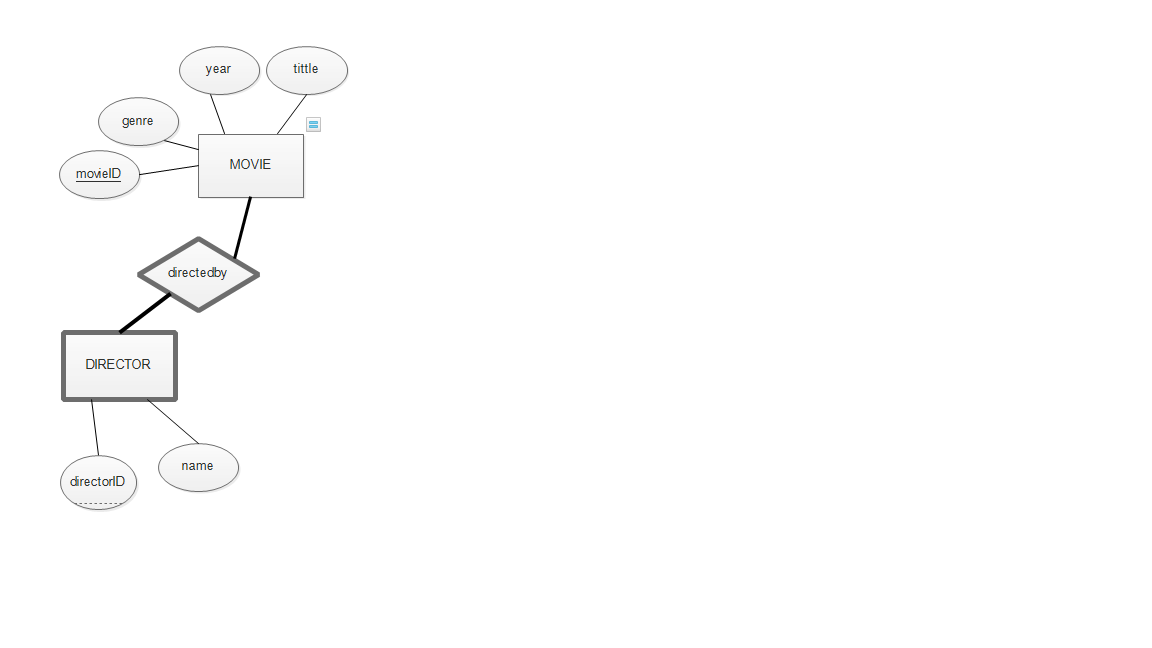
\includegraphics[scale=0.3]{movie-director.png}
Explanation related to user scenario: movie directed by director relation , weak entity.
when movie gets deleted we take everything that comes with that movie, director.
For the first moviegoer scenario, selecting a movie. The movie relation is used in the diagram, it has the attributes that a user would need. The movie table would have movieID, genre, year, and title and director has name and director ID
when selecting a movie you can also select by director 
\item{ }
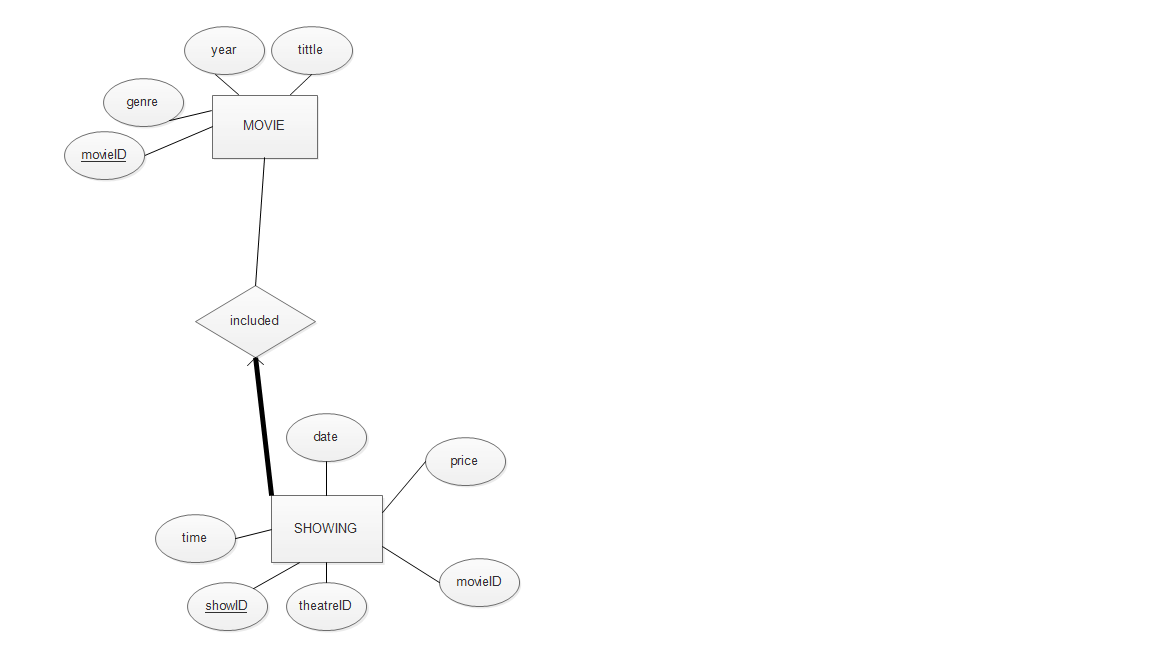
\includegraphics[scale=0.3]{MovieofShowing.png}
explanation related to user scenario: showing of one movie. For the ticket seller scenario, he/she is approached by a moviegoer who purchased the wrong ticket for the wrong showing. Showing has attributes that would enable this transaction. 
\item{ }
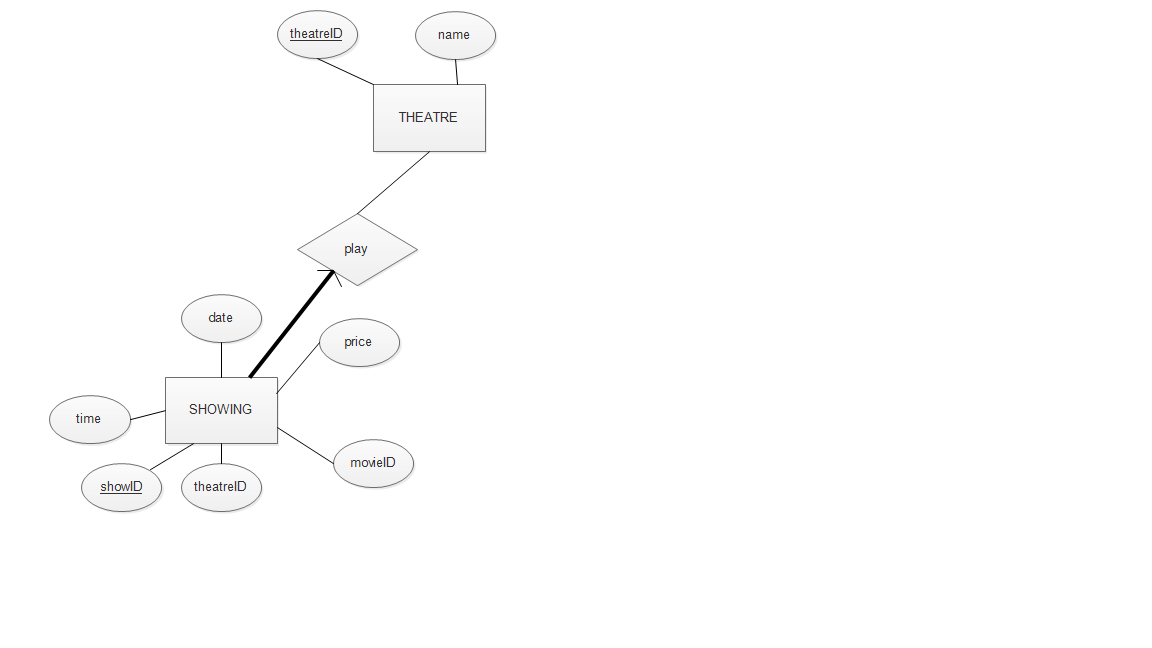
\includegraphics[scale=0.3]{ShowingPlayedinTheatre.png}
explanation related to user scenario: For the showing manager scenario , it states that the theater manager has the ability to remove a showtime of a movie. this relation shows theater attributes and showing attributes that can allow the showing manager to remove showtimes 
\item{ }
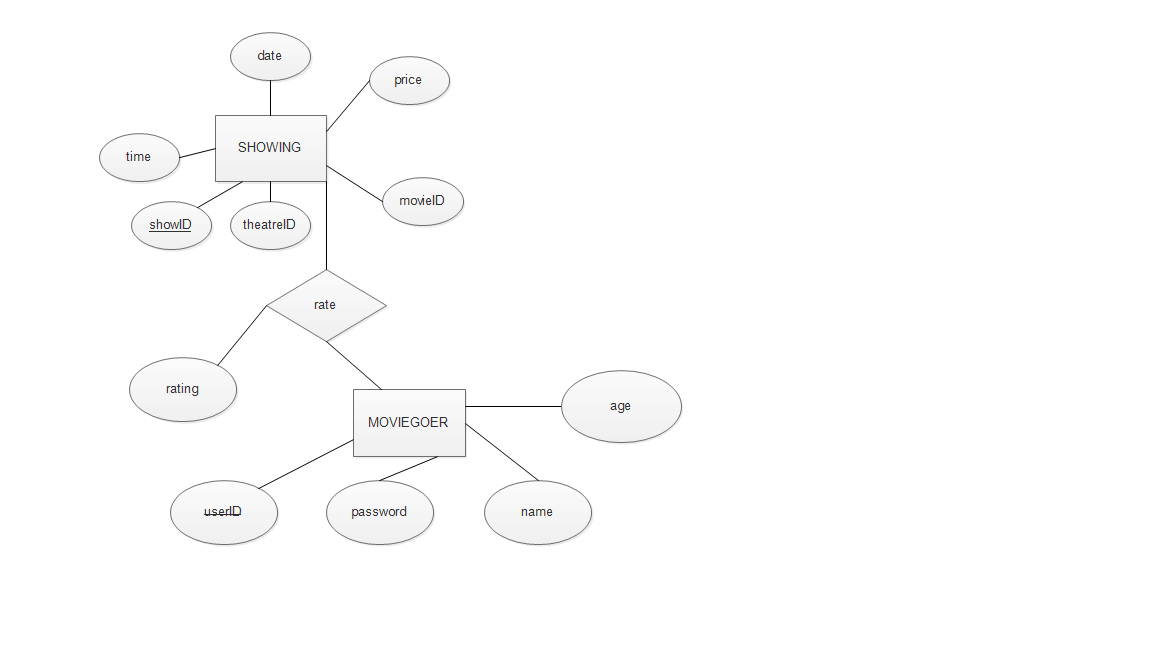
\includegraphics[scale=0.3]{MoviegoerrateShowing.png}
explanation related to user scenario: moviegoer can rate showing , each of their attributes allow a user to rate a showing by movie ID 
\item{ }
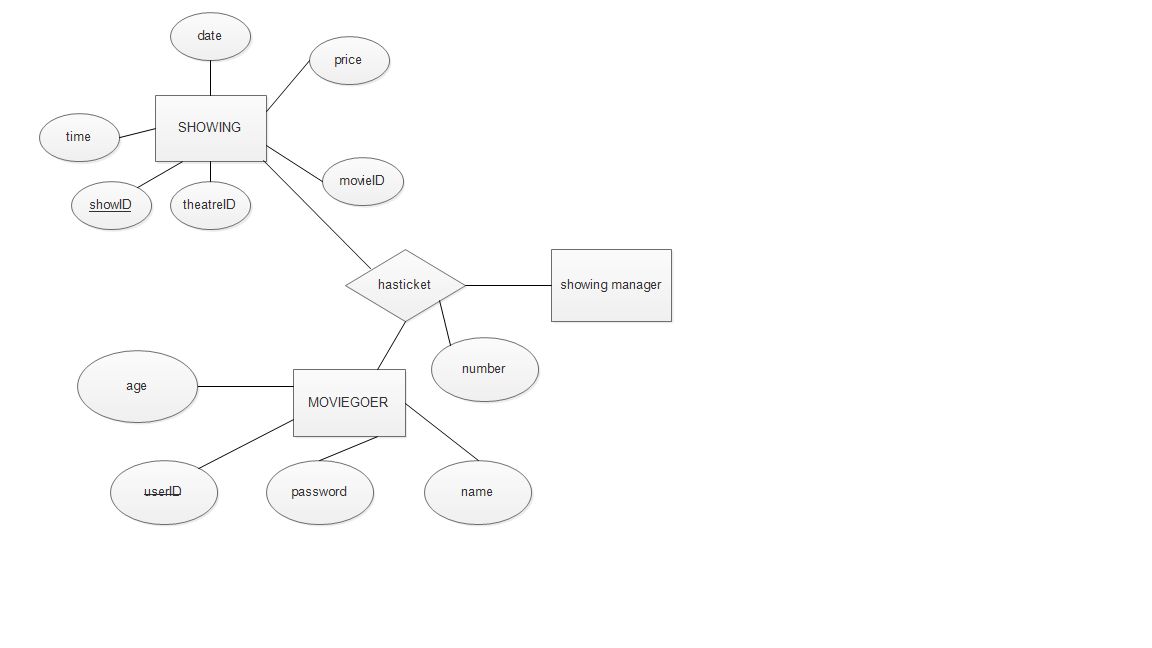
\includegraphics[scale=0.3]{MoviegoerhasticketShowing.png}
explanation related to user scenario: This ternary relationship is between ticket seller  , moviegoer and showing . For the ticket seller scenario, he/she is approached by a moviegoer who purchased the wrong ticket for the wrong showing.The ticket seller has access to the user accounts, and it is depicted in the relationship has ticket between showing and moviegoer because the tickets seller has all tickets of the moviegoer and is able to change it.
\item{ }
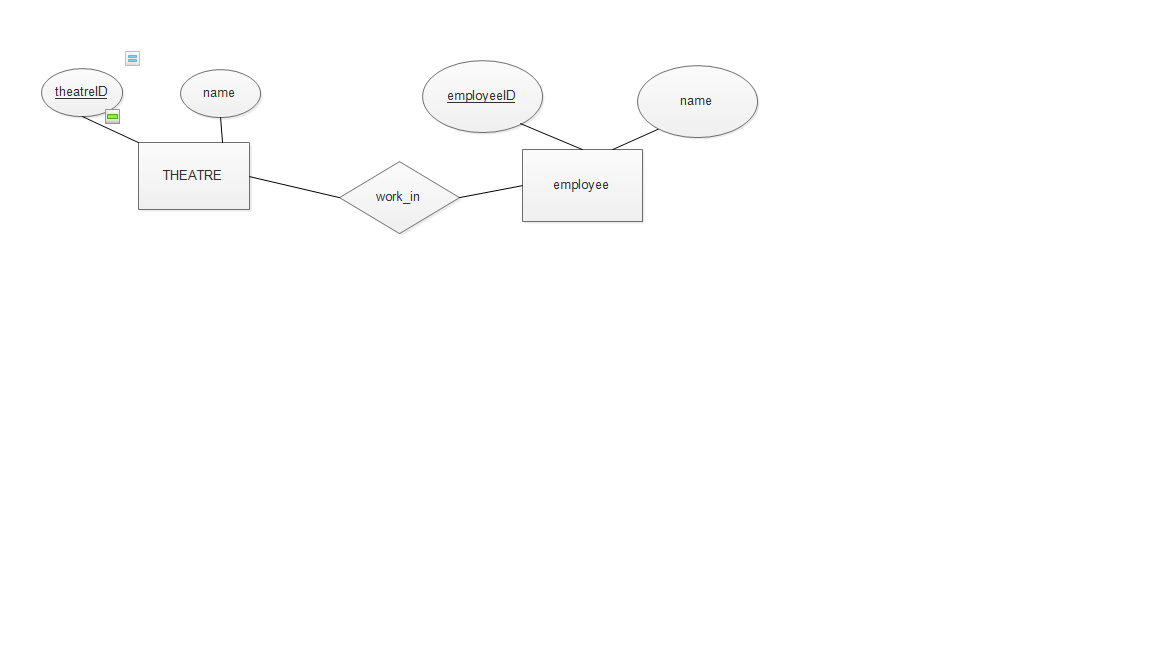
\includegraphics[scale=0.3]{TheatrehasEmployee.png}
explanation related to user scenario: many employees work in each theater ,relationship called employeeWorkin, the most important employees being ticket seller, chain manager, showing manager, and theater manager
\item{ }
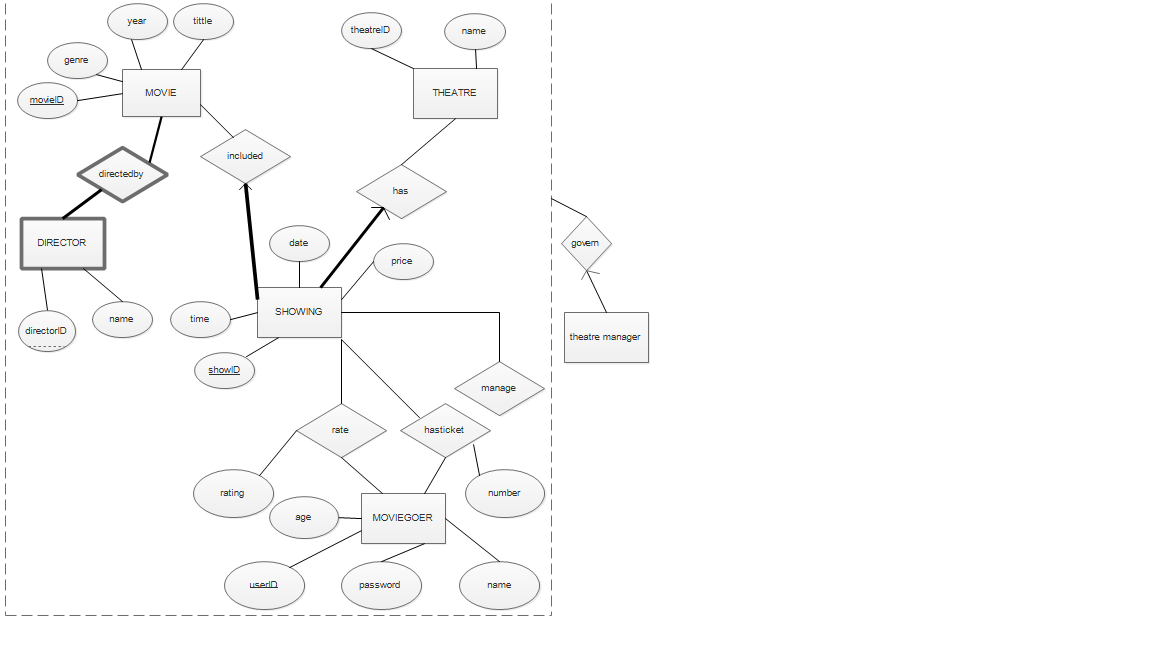
\includegraphics[scale=0.3]{theatremanagergovern.png}
explanation related to user scenario: a theatre manager of that theatre can manage all the stuff in that theatre, including showing, movie, and moviegoer.
\item{ }
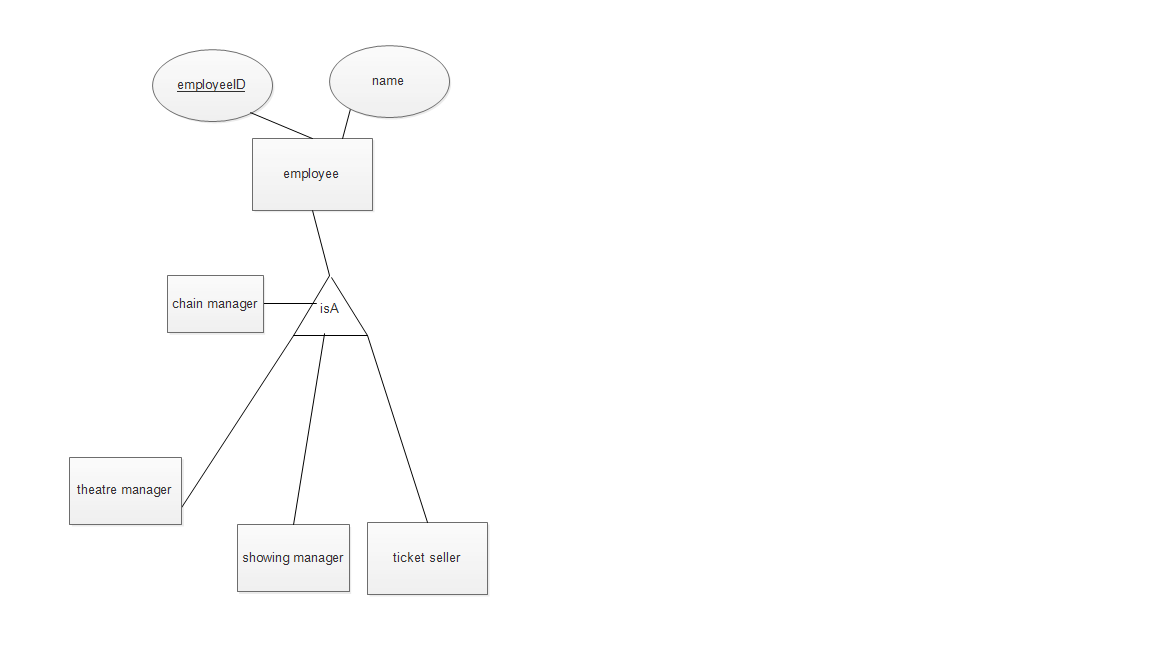
\includegraphics[scale=0.3]{isA.png}
explanation related to user scenario: ticket seller, chain manager, showing manager, and theater manager are different types of employee. Each of them has different authority
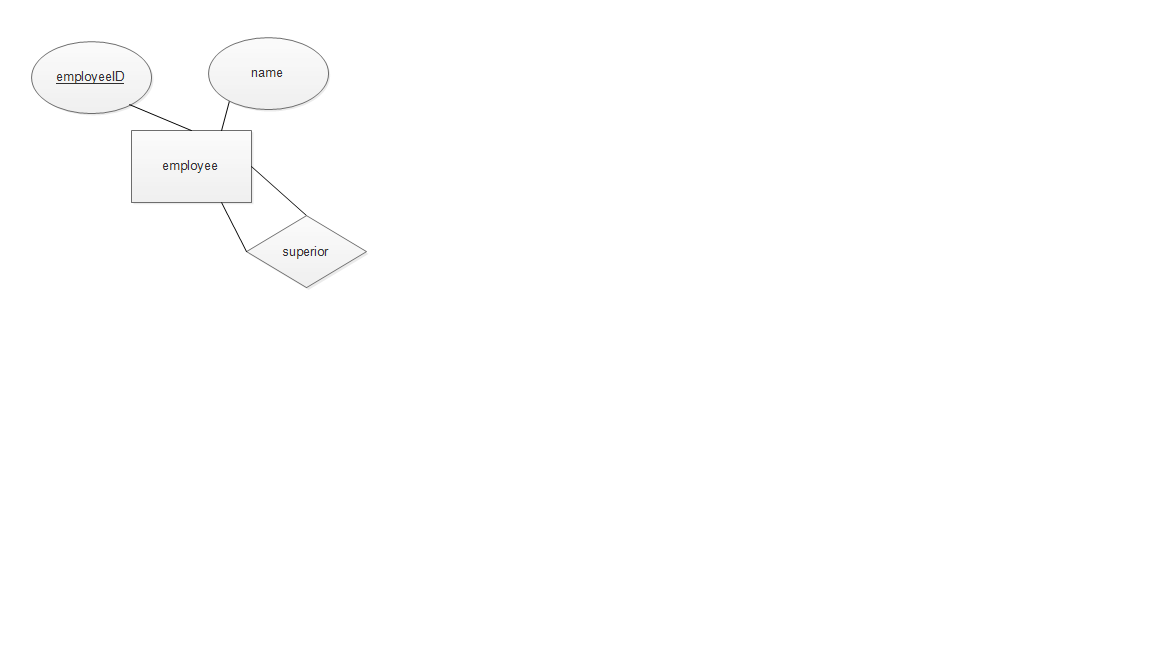
\includegraphics[scale=0.3]{superior.png}
explanation related to user scenario: each employee may be superior to other employees. It's a unary relationship.
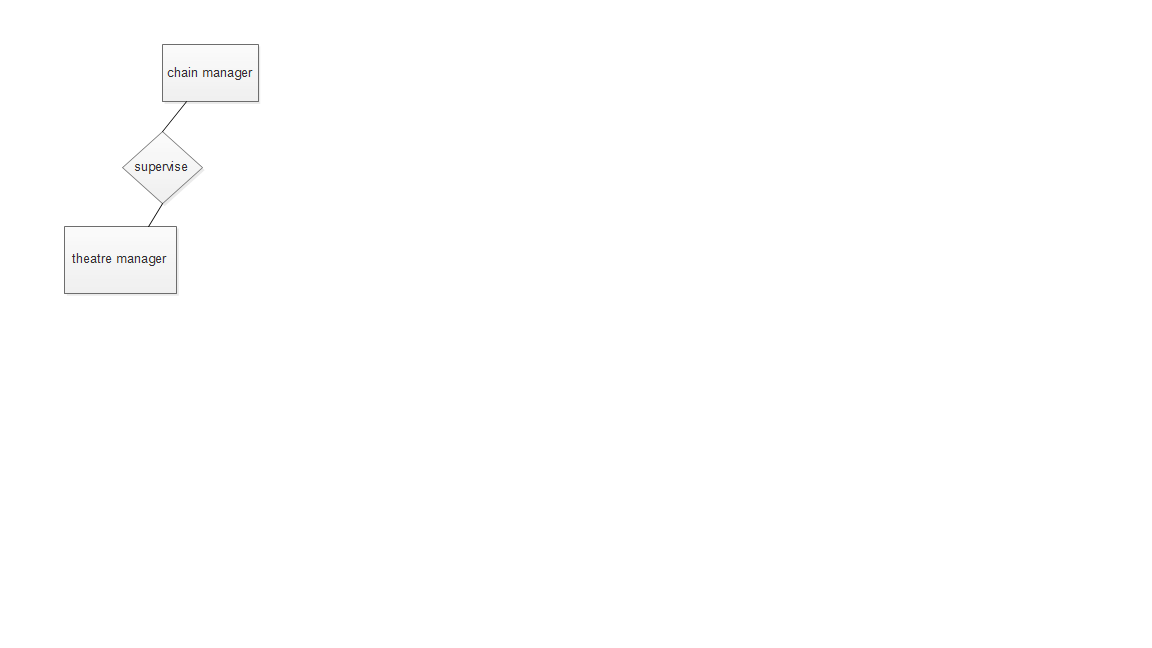
\includegraphics[scale=0.3]{supervise.png}
explanation related to user scenario: Chain manager supervise all the theatre manager in that chain.
\end{itemize}
\begin{itemize} 
\item{ The ER diagram in its entirety: }
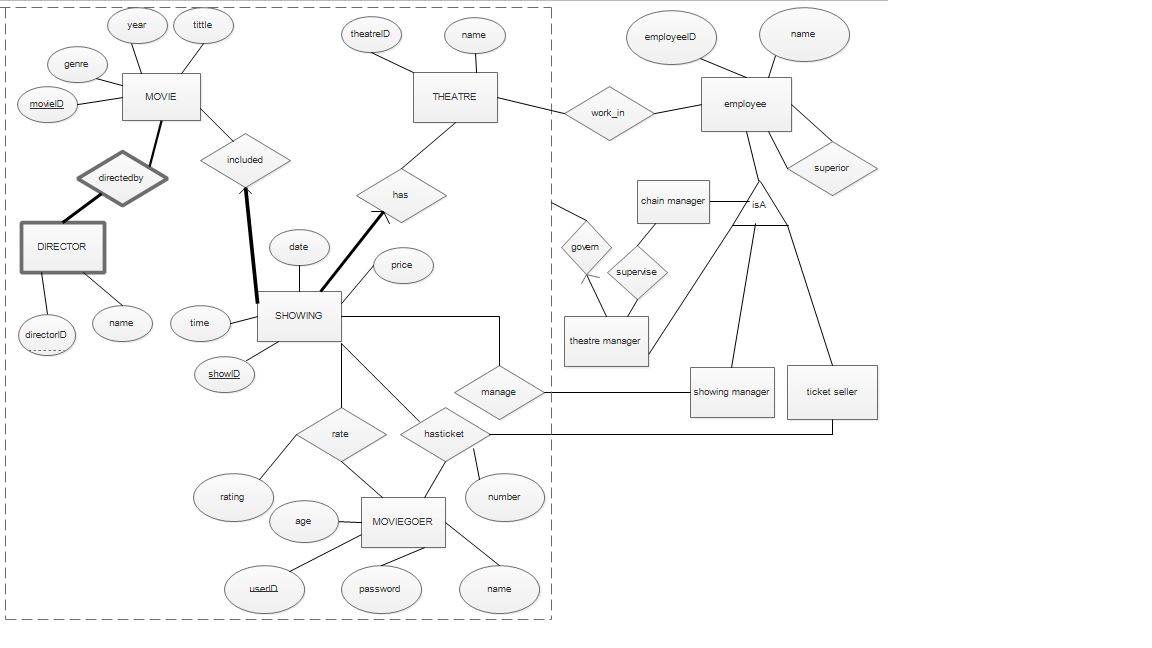
\includegraphics[scale=0.3]{ERmodel.png}
\item{ The ER diagram description (corresponding to the user scenarios): }
For the moviegoer scenario the moviegoer logs into his/her account and selects a movie and buys ticket(s). The relationship between showing and moviegoer depicts this relationship. The attributes in showing are needed to buy a ticket. The attributes for showing are time, showID, theaterID, movieID, price, and date and each attribute is used in this transaction.For selecting a movie the movie relation is used in the diagram, it has the attributes that a user would need. The movie table would have movieID, genre, year, and title.The relationship between moviegoer and showing displays that the moviegoer has a ticket for the chosen showing the moviegoer picked. The moviegoer's attributes are what we need to make this happen , which leads into the second user scenario.
For the moviegoer to register in our system we would need the userID, password, and name. To buy a ticket a user would have to register in the system therefore these attributes for moviegoer are important.
\item{ }
For the chain manager scenario , the chain manager adds employees to the database. The relationship between employee and theater depicts this scenario. The employee relation has an attribute ,employeeID. which is essential to this scenario because the theater has lots of employees working for them but every person working for the theaters are employees, that is why we use the is A relationship between them all , if not a theater manager , ticket seller, or administrator then its just a regular employee which is the other employees working at the theatre.
For the second scenario , it states that the showing manager has the ability to remove a showtime of a movie, the manage relationship between showing and theater manager, the attributes for the showing relation has time and date and it can be changed by the theater manager.
\item{ }
For the ticket seller scenario, he/she is approached by a moviegoer who purchased the wrong ticket for the wrong showing.The ticket seller has access to the user accounts, and it is depicted in the relationship has ticket between showing and moviegoer because the tickets seller has all tickets of the moviegoer and is able to change it.
For the second scenario, it states that the ticket seller wants to see if  a particular movie is doing well. The ticket seller is able to do this because he/she has access , by the has tickets relationship, to the showing table, where he/she can look up a movie and its ticket sales
\item{ }
For the theater manager scenario, the first scenario states that the theater manager taking out all showings of a certain movie. For this the theater manager has needs and has access to ticket sales, and showings. The theater manager is the administrator and has access to everything, relations such as movie, director, showing, theater,and moviegoer and employees because of the relationship between theater and employees. Theres an aggregation in the diagram to depict this administrator manage relationship.
The second scenario for the chain manager/administrator is he/she wants to see if a movie showing in one theater is worth showing in other branches. Again the administrator has access to information of all cinemas. in the showing relation the admin has access to rating because of the rate relationship between moviegoer and showing which has an attribute of rating. Therefore the administrator can find out the ratings of any showing as well as ticket sales because of the has ticket relationship and its number attribute which is between showing and moviegoer.
\item{ The integrity constraints defined in the ER diagram: }
Please insert the integrity constraints in here:
\begin{itemize} 
\item{ Integrity Constraint: }
Each showing must be of exactly one movie.
\item{ The description and justification of the integrity constraint: }
 A showing, by definition, is a specific movie being shown in a specific place at a specific time.  By this definition, there has to be a movie to be shown.  There cannot be more than one movie because an audience does not watch multiple movies at once.
\end{itemize}
\begin{itemize} 
\item{ Integrity Constraint: }
Each showing has exactly one theater.
\item{ The description and justification of the integrity constraint: }
 A showing, by definition, is a specific movie being shown in a specific place at a specific time.  The theater is that specific place, and so there can only be one.  And there has to be one, because there needs to be somewhere for the movie to be shown.
\end{itemize}
\begin{itemize} 
\item{ Integrity Constraint: }
Each movie has at least one director.
\item{ The description and justification of the integrity constraint: }
Every movie that exists was directed by someone.  However, it is possible for multiple people to co-direct.
\end{itemize}
\begin{itemize} 
\item{ Integrity Constraint: }
Each director has at least one movie.
\item{ The description and justification of the integrity constraint: }
 By definition, to be a director that person must have directed something.  Furthermore, there is no reason to store a director unless they belong to a movie the theater is storing information on.  It is possible for a director to have directed multiple movies.
\end{itemize}
\begin{itemize} 
\item{ Integrity Constraint: }
movieID is the primary key for a movie.
\item{ The description and justification of the integrity constraint: }
All entities need a key, and no movie trait is guaranteed to be unique (two movies can share a title, for example), so a unique ID number needs to be created for each movie.
\end{itemize}
\begin{itemize} 
\item{ Integrity Constraint: }
showId is the primary key for a showing.
\item{ The description and justification of the integrity constraint: }
All entities need a key, and no showing trait is guaranteed to be unique- one theater could have two showings of the same movie at the same time.  For this reason, a unique ID number needs to be created for each showing.
\end{itemize}
\begin{itemize} 
\item{ Integrity Constraint: }
userID is the primary key for a moviegoer.
\item{ The description and justification of the integrity constraint: }
All entities need a key, and no moviegoer trait is guaranteed to be uniquie (two moviegoers can have the same name, for example), so a unique ID number needs to be created for each moviegoer.
\end{itemize}
\begin{itemize} 
\item{ Integrity Constraint: }
theaterID is the primary key for a theater.
\item{ The description and justification of the integrity constraint: }
All entities need a key.  Since there is no other information stored for a theater that is uniquely identifying, so an ID number must be created for that purpose.
\end{itemize}
\begin{itemize} 
\item{ Integrity Constraint: }
employeeID is the primary key for an employee.
\item{ The description and justification of the integrity constraint: }
Just like with moviegoers, it is possible for multiple employees to share a name or other attributes, so a unique ID number is necessary for each employee
\end{itemize}
\begin{itemize} 
\item{ Integrity Constraint: }
Each theater manager can manage at most one theater.
\item{ The description and justification of the integrity constraint: }
 A manager of multiple theaters is a different job (admin).  A manager typically manages exactly one theater, but it is possible for a manager to not yet be assigned a theater, or to be a substitute and not belong to a specific theater.
\end{itemize}
\end{itemize}
}
